% ======================================================================
\chapter{Methodology}

\section{Tools and Techniques}
\begin{itemize}
\item \textbf{TF-IDF}~\cite{salton1988term} gives a term a high weight when it is frequent in the message but uncommon in the collection. In the main detector we join word 1--2-grams with character 2--5-grams. The cross-domain study keeps them apart: word 1--2-grams on one side, character 3--5-grams on the other.
\item \textbf{Logistic regression} is a linear model, so its coefficients can be read directly: each one says how strongly a word pulls a message towards scam or towards genuine.
\item \textbf{Multinomial Naive Bayes} learns how often each term appears in each class and then applies Bayes' rule. It serves as the classical baseline in the cross-domain study.
\item \textbf{MinHash and locality-sensitive hashing}~\cite{broder1997resemblance} find messages that are nearly identical, which lets us group them into campaigns.
\item \textbf{Confident learning}~\cite{northcutt2021confident} tells us which labels to re-read: the ones a cross-validated model strongly disagrees with.
\item \textbf{Intent rules written as regular expressions} spot requests for an OTP, ``pay to receive'' offers, remote-access apps and legal threats, as well as reassuring signals such as ``do not share your OTP''.
\item \textbf{Supervised domain adaptation} here simply means adding a labelled sample of target messages to the source training data~\cite{daume2007frustratingly,pan2010survey}.
\item \textbf{Bootstrap intervals, mean $\pm$ SD across seeds and McNemar's test}~\cite{mcnemar1947note,dietterich1998approximate} show how certain each result is and whether two models differ on the same messages.
\item \textbf{Software:} scikit-learn~\cite{pedregosa2011scikit} for the models, ftfy to fix broken text encodings, and FastAPI, Next.js and Streamlit for the applications.
\end{itemize}

\section{Data Set with Explanation}

\subsection{ScamGuard-IN-2026 (main detector)}
Indian scams and genuine Indian service messages use largely the same words, and public smishing data offers only reported messages whose labels nobody checked. We therefore assembled our own corpus, ScamGuard-IN-2026, with real genuine Indian messages, verified labels and the scam types seen in 2025--26. Its sources are listed in Table~\ref{tab:sources}.

\begin{table}[H]
\centering
\caption{Sources of ScamGuard-IN-2026}
\label{tab:sources}
\small
\begin{tabular}{|L{3.6cm}|L{2.1cm}|L{1.4cm}|L{1.2cm}|L{3.6cm}|}
\hline
\textbf{Source} & \textbf{Licence} & \textbf{Genuine} & \textbf{Scam} & \textbf{Use} \\
\hline
R1: IMC 2025 smishing collection, India subset, audited~\cite{agarwal2025fishing} & CC BY 4.0 & 963 & 3,987 & train, development, test \\
\hline
R2: India Spam SMS collection, audited~\cite{indiasms2024} & MIT & 1,694 & 6 & train, development, test \\
\hline
R3: 2025--26 advisory and news texts & Quoted with source & 1 & 11 & test only \\
\hline
S: Synthetic templates & Project & 2,950 & 1,787 & training only \\
\hline
\textbf{Total} & & \textbf{5,608} & \textbf{5,791} & \textbf{11,399 messages} \\
\hline
\end{tabular}
\end{table}

\textbf{Checking the labels.} Everything in the IMC 2025 collection is something a user \emph{reported}, which is not the same as a confirmed scam. We took 2,922 decisions over the groups of reported near-duplicates. In 1,253 cases a rule settled it: the message carried a strong fraud cue (an account threat with a KYC instruction, a prize that needs a fee, a request for an OTP) and nothing that suggested a genuine sender; a spot check of 40 of these found no mistake. The remaining 1,669 we read one at a time and marked 583 as scam, 867 as genuine and 219 as unclear; the unclear ones were dropped. As a second pass, a cross-validated model pointed to 44 rows whose labels it strongly disagreed with. Re-reading them led to 19 corrections and 7 removals. In the end, 963 of the 4,950 IMC rows we kept (19.5\%) are genuine messages.

\textbf{Campaigns and splits.} Two messages fall into one campaign if the Jaccard similarity of their word 3-shingles, estimated with MinHash, reaches 0.6. This turns the 6,662 real messages into 4,085 campaigns. A hash of each campaign's first message then sends the whole campaign to training (60\%), development (15\%) or test (25\%); Table~\ref{tab:splits} gives the counts.

\begin{table}[H]
\centering
\caption{ScamGuard-IN-2026 splits}
\label{tab:splits}
\begin{tabular}{|l|r|r|l|}
\hline
\textbf{Split} & \textbf{Genuine} & \textbf{Scam} & \textbf{Content} \\
\hline
Train & 4,581 & 4,064 & real and synthetic \\
\hline
Development & 361 & 507 & real only \\
\hline
Test & 665 & 1,209 & real only, unseen campaigns \\
\hline
2026 test & 1 & 11 & advisories \\
\hline
\end{tabular}
\end{table}

\subsection{Datasets of the cross-domain study}
Our guide named both datasets. \textbf{Dataset A, the source,} is the UCI SMS Spam Collection~\cite{almeida2011contributions}, released under CC BY 4.0. It holds 5,574 messages from the UK (4,827 ham, 747 spam) and is described in the paper that introduced it. \textbf{Dataset B, the target,} is the India Spam SMS Classification set~\cite{indiasms2024}, published in 2024 under the MIT licence. Its 2,267 rows have two fields, \texttt{Msg} and \texttt{Label}, with 1,522 ham and 745 spam. People submitted the messages through an online form, and the repository says nothing about how labels were assigned.

\textbf{What the audit found.} Dataset B contained one empty message and 204 exact repeats. In 176 rows the emoji and punctuation had been saved as garbled bytes, and in 40 rows the Devanagari text had been turned into question marks that cannot be recovered. We found no message carrying two different labels. Reading ten random messages from each class, the labels looked reasonable: the spam is mostly operator, bank and shop promotions with a link, and the ham is mostly short personal or group-chat text. Only one message, ``ok'', appeared in both datasets, and we removed it from B.

\textbf{Cleaning.} Both datasets went through identical steps. Labels became spam = 1 and ham = 0, unusable rows were dropped, garbled encodings were fixed with ftfy, everything was lowercased, runs of spaces were collapsed and exact repeats were removed. We left URLs, numbers and punctuation in place, since they are often what gives spam away. Table~\ref{tab:xdata} shows the counts after each dataset was cleaned; Figures~\ref{fig:classdist} and~\ref{fig:lendist} show the class balance and message lengths.

\begin{table}[H]
\centering
\caption{Cross-domain datasets before and after cleaning}
\label{tab:xdata}
\begin{tabular}{|l|r|r|r|r|r|}
\hline
\textbf{Dataset} & \textbf{Raw} & \textbf{Clean} & \textbf{Ham} & \textbf{Spam} & \textbf{Spam \%} \\
\hline
A: UCI SMS Spam Collection & 5,574 & 5,158 & 4,517 & 641 & 12.4 \\
\hline
B: India Spam SMS & 2,267 & 2,050 & 1,314 & 736 & 35.9 \\
\hline
\end{tabular}
\end{table}

\begin{figure}[H]
\centering
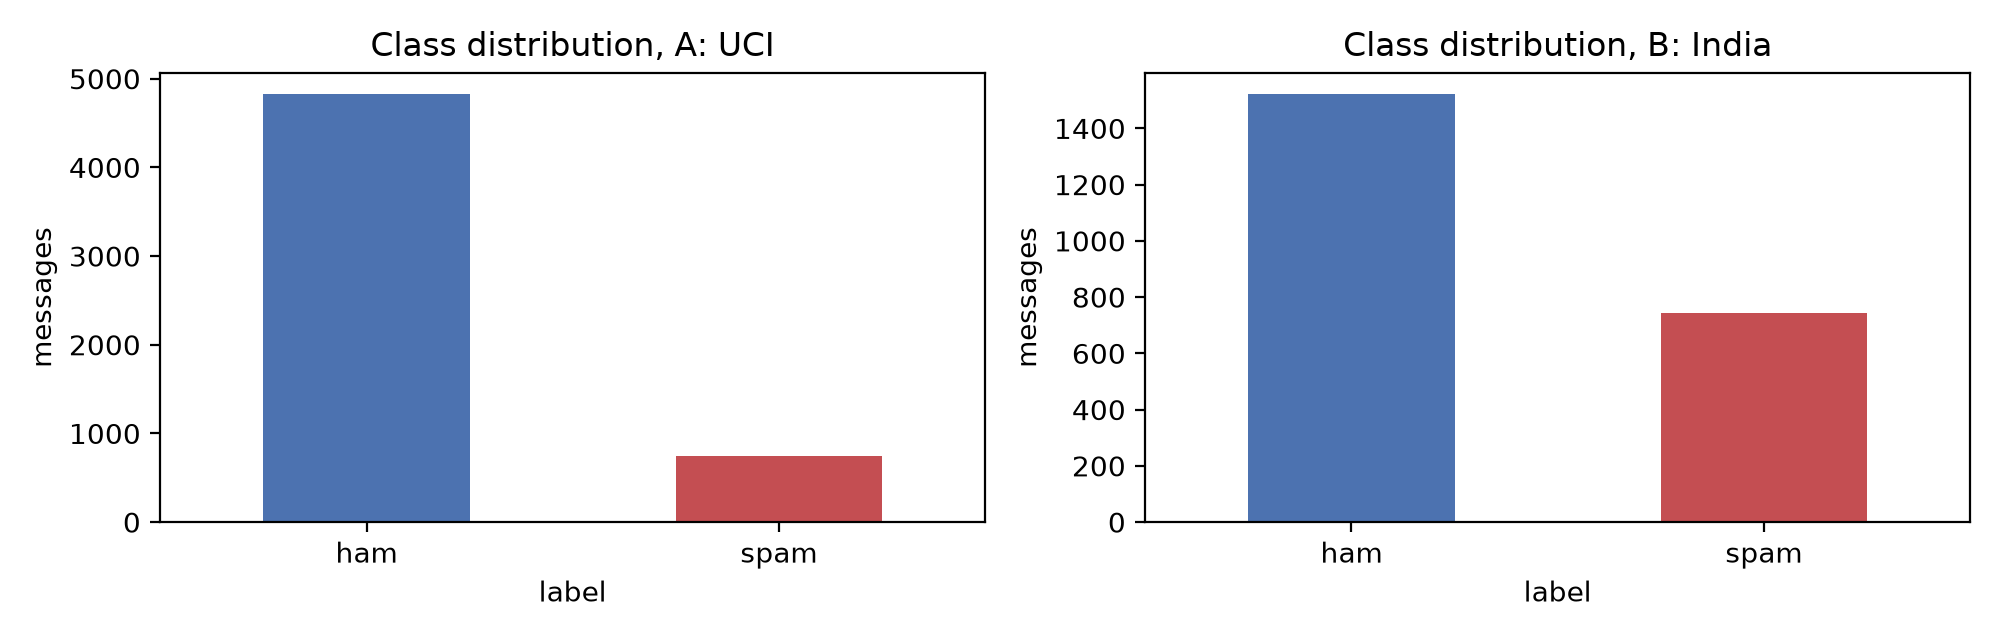
\includegraphics[width=0.85\linewidth]{figures/fig1_class_distribution.png}
\caption{Class distribution of Dataset A (UCI) and Dataset B (India) before cleaning}
\label{fig:classdist}
\end{figure}

\begin{figure}[H]
\centering
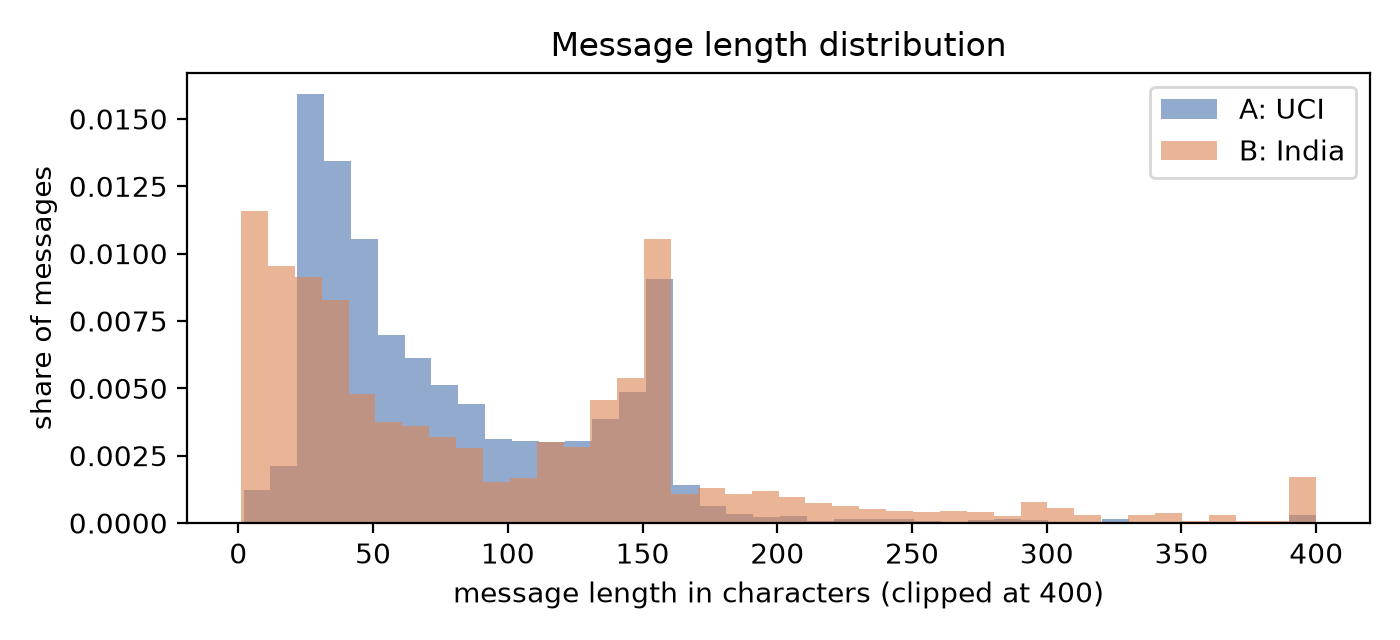
\includegraphics[width=0.65\linewidth]{figures/fig2_length_distribution.png}
\caption{Message length distribution of the two datasets}
\label{fig:lendist}
\end{figure}

\section{Flowchart of Methodology from Start to End}
The two pipelines are drawn separately: Figure~\ref{fig:flow} covers the main detector and Figure~\ref{fig:xflow} the cross-domain study.

\begin{figure}[H]
\centering
\begin{tikzpicture}[node distance=5mm,
  box/.style={draw, rounded corners=2pt, align=center, font=\small, minimum width=6.5cm, minimum height=8mm, fill=white},
  arr/.style={-{Stealth[length=2.2mm]}, thick}]
\node[box] (a) {Collect sources: IMC 2025 India subset, India SMS,\\2025--26 advisories, team SMS, synthetic templates};
\node[box, below=of a] (b) {Normalise anonymised entities and mask personal data};
\node[box, below=of b] (c) {Group near-duplicates into campaigns (MinHash LSH)};
\node[box, below=of c] (d) {Audit labels: rule-confirmed, manual review,\\second pass on model disagreements};
\node[box, below=of d] (e) {Split by campaign: train / development / test};
\node[box, below=of e] (f) {Preprocess: clean, tokenise (Latin + Devanagari)};
\node[box, below=of f] (g) {TF-IDF word + character features; train classifiers};
\node[box, below=of g] (h) {Select model on development split; evaluate on test};
\node[box, below=of h] (i) {Register the trained model; serve with intent rules and explanations};
\node[box, below=of i] (j) {Deploy web application; daily live-site check};
\foreach \x/\y in {a/b,b/c,c/d,d/e,e/f,f/g,g/h,h/i,i/j} \draw[arr] (\x) -- (\y);
\end{tikzpicture}
\caption{Flow of the methodology}
\label{fig:flow}
\end{figure}

\begin{figure}[H]
\centering
\begin{tikzpicture}[node distance=5mm,
  box/.style={draw, rounded corners=2pt, align=center, font=\small, minimum width=7cm, minimum height=8mm, fill=white},
  arr/.style={-{Stealth[length=2.2mm]}, thick}]
\node[box] (a) {Load Dataset A (UCI, source) and Dataset B (India, target)};
\node[box, below=of a] (b) {Audit: counts, missing values, duplicates, encoding, labels, provenance};
\node[box, below=of b] (c) {Clean both the same way; remove duplicates and A--B overlap};
\node[box, below=of c] (d) {Split A 80/20; split B 70/30 into adaptation pool and final test};
\node[box, below=of d] (e) {Word and character TF-IDF; choose $\alpha$, $C$ on A-train only};
\node[box, below=of e] (f) {Train NB and LR on A-train; test on A-test and on B (cross-domain)};
\node[box, below=of f] (g) {Add 10\%, 20\%, 40\% of the pool; refit; test on the same B-test};
\node[box, below=of g] (h) {Repeat for seeds 42, 123, 2026; mean $\pm$ SD; McNemar test};
\node[box, below=of h] (i) {Near-duplicate check; manual error analysis};
\node[box, below=of i] (j) {Save baseline and adapted models; serve in the web app and Streamlit};
\foreach \x/\y in {a/b,b/c,c/d,d/e,e/f,f/g,g/h,h/i,i/j} \draw[arr] (\x) -- (\y);
\end{tikzpicture}
\caption{Flow of the cross-domain study}
\label{fig:xflow}
\end{figure}

\section{Explanation of Methodology in detail with Equations and Formulae}

\subsection{Problem definition}
Given a message $x$, the detector produces a score $s(x)\in[0,1]$ and decides
\begin{equation}
\hat{y}=\begin{cases}1 \;(\text{scam/spam}) & \text{if } s(x)\ge 0.5\\ 0 \;(\text{legitimate/ham}) & \text{otherwise.}\end{cases}
\end{equation}

\subsection{Preprocessing}
The main detector's cleaner swaps e-mail addresses, URLs (bare ones like \texttt{bit.ly/x} included) and phone numbers for placeholder tokens. It then lowercases the text, strips punctuation without damaging Devanagari vowel signs, and turns any other number into a number token. The tokenizer keeps Latin and Devanagari words, drops English stop words and trims common suffixes. Take \textit{``Dear customer, your SBI account will be blocked today. Update your KYC at http://sbi-kyc.xyz and share the OTP''}: it comes out as \texttt{dear customer sbi account will block today update kyc \_\_url\_\_ share otp}. Training and the live service call the very same code. One side effect is worth stating: since punctuation and digits disappear before features are built, spellings such as \textit{K.Y.C} or \textit{bl0cked} lose their keyword, and such messages have to be caught by their other words or by the intent rules. The cross-domain study cleans far less, as the guide asked. It only lowercases and tidies whitespace, so URLs, numbers and punctuation stay; the word vectorizer splits on punctuation, while the character vectorizer sees it.

\subsection{Feature extraction}
For a term $t$ in message $d$, with $N$ training messages and document frequency $\mathrm{df}(t)$, the TF-IDF weight is
\begin{equation}
w_{t,d}=g(\mathrm{tf}_{t,d})\cdot\left(\ln\frac{1+N}{1+\mathrm{df}(t)}+1\right),
\end{equation}
after which each message vector is scaled to unit length. For the main detector $g$ is sublinear, $g(\mathrm{tf})=1+\ln\mathrm{tf}$, and the vocabulary has word 1--2-grams (at most 30,000) plus character 2--5-grams (at most 60,000); pruning leaves 35,148 features. The cross-domain study uses plain counts, $g(\mathrm{tf})=\mathrm{tf}$, and either word 1--2-grams (at most 20,000) or character 3--5-grams taken inside word boundaries. No vectorizer ever sees anything but training data.

\textit{A small example.} Take three messages: ``update kyc now'', ``kyc update otp'' and ``order delivered today'', so $N=3$. In the first one, \textit{update} and \textit{kyc} each occur in two messages ($\mathrm{df}=2$) and \textit{now} in one, giving IDF values of $\ln(4/3)+1=1.288$ and $\ln 2+1=1.693$. Normalised, the vector is $(0.518, 0.518, 0.681)$, so the word that is rarest in the collection gets the most weight.

\subsection{Logistic regression}
Logistic regression estimates
\begin{equation}
p(x)=\sigma\!\left(\mathbf{w}^{\top}\phi(x)+b\right)=\frac{1}{1+e^{-(\mathbf{w}^{\top}\phi(x)+b)}},
\end{equation}
by minimising the class-weighted, $\ell_2$-regularised log-loss
\begin{equation}
\min_{\mathbf{w},b}\;\frac{1}{2}\|\mathbf{w}\|^2 + C\sum_{i=1}^{n}\alpha_{y_i}\Big[-y_i\ln p(x_i)-(1-y_i)\ln\big(1-p(x_i)\big)\Big],
\end{equation}
where the class weights are $\alpha_c=n/(2n_c)$. We set $C=16$ for the main detector. In the cross-domain study $C$ came from cross-validation on the source training data: 100 for word features and 10 for character features. The trained main model has bias $b=-4.82$. Among its strongest weights, \textit{prize} ($+2.98$), \textit{will block} ($+2.87$) and \textit{kyc} ($+2.69$) push towards scam, while \textit{branch} ($-2.22$) and \textit{not share} ($-1.85$) push towards genuine. The SBI message from the preprocessing example gets $z=\mathbf{w}^\top\phi(x)+b=8.99$, so $p=0.9999$. A real OTP alert, ``482913 is your OTP for Rs 2,499 at Amazon. Do not share it with anyone'', gets $z=-5.53$ and $p=0.004$.

\subsection{Multinomial Naive Bayes}
Naive Bayes predicts the class with the larger posterior,
\begin{equation}
\hat{c}=\arg\max_{c\in\{0,1\}}\Big[\ln P(c)+\sum_{t} x_t \ln P(t\mid c)\Big],\qquad P(t\mid c)=\frac{N_{tc}+\alpha}{N_c+\alpha|V|},
\end{equation}
Here $x_t$ is the TF-IDF value of term $t$, $N_{tc}$ is the summed weight of $t$ in class $c$, $N_c$ is the summed weight of all terms in $c$, $|V|$ is the vocabulary size and $\alpha$ is the smoothing constant. Cross-validation on source training data picked $\alpha=0.03$. We also report the library default, $\alpha=1$, because the difference turns out to matter a great deal.

\subsection{Intent evidence and fusion}
The rule layer has 31 patterns for 26 scam intents, each with a weight $w_i$ that we set by hand, and ten protective signals with weights $v_j$. Let $E^{+}=\sum_{i\in I(x)}w_i$, halved if only weak context cues fire, and $E^{-}=\sum_{j\in P(x)}v_j$, halved if $E^{+}\ge 0.5$. The final score is then
\begin{equation}
s(x)=\sigma\!\Big(\operatorname{clip}\big(\operatorname{logit}p(x),-4,4\big)+5\,(E^{+}-E^{-})\Big),
\end{equation}
If a message is shaped like a genuine transaction alert or service notice and has no blocking cue, the score is capped at 0.15. A separate ``decoy'' rule handles the trick of writing ``never share your OTP'' and then asking for it anyway.

\subsection{Near-duplicate grouping}
After links and digits are replaced, a message is reduced to $S$, the set of its word 3-shingles. Two messages share a campaign if
\begin{equation}
J(S_1,S_2)=\frac{|S_1\cap S_2|}{|S_1\cup S_2|}\ \ge\ 0.6,
\end{equation}
where $J$ is estimated from 96 MinHash permutations with locality-sensitive hashing.

\subsection{Domain adaptation}
Write $A_{train}$ for the source training split, $P$ for the target adaptation pool and $S_f\subset P$ for a stratified sample of size $|S_f|=\lfloor f\,|P|\rfloor$. The adapted model learns from
\begin{equation}
D_f=A_{train}\cup S_f,\qquad f\in\{0, 0.1, 0.2, 0.4\},
\end{equation}
and the vectorizer is fitted again on $D_f$, which lets Indian words into the vocabulary. The pool has $|P|=1{,}435$ messages, so the three samples hold 143, 287 and 574. All values of $f$ are scored on one fixed target test set, $B_{test}$, of 615 messages.

\subsection{Evaluation metrics}
Scam (or spam) is the positive class throughout:
\begin{align}
\text{Accuracy}&=\frac{TP+TN}{TP+TN+FP+FN}, & \text{Precision}&=\frac{TP}{TP+FP},\\
\text{Recall}&=\frac{TP}{TP+FN}, & F_1&=\frac{2\cdot\text{Precision}\cdot\text{Recall}}{\text{Precision}+\text{Recall}},\\
\text{False-alarm rate}&=\frac{FP}{FP+TN}. & &
\end{align}
We draw confidence intervals from 1,000 bootstrap resamples, and when an experiment is repeated over seeds we give the mean $\pm$ standard deviation.

\subsection{Statistical test}
When two models are scored on the same messages, only the messages they disagree on carry information. Let $b$ count those that only the first model gets right and $c$ those that only the second gets right. If the two models were equally good, $\min(b,c)$ would follow a binomial distribution with $n=b+c$ and probability $0.5$. The exact McNemar test~\cite{mcnemar1947note,dietterich1998approximate} turns this into a two-sided $p$-value.
